%!TEX root = main.tex

%%%%%%% SECTION %%%%%%%
\section{Modèle événementiel pour l'intégration du domaine 3D dans les 
EVC}

%\subsection{Introduction}
La méthodologie orientée événements intègre plusieurs aspects souvent laissés 
de côté dans la littérature concernant le développement des environnements 
virtuels collaboratifs pour la visualisation et la manipulation d'objets 3D. 
Les événements peuvent en effet être utilisés dans le cadre de \gls{CSCW} et 
d'\gls{EVC}, qui ont évolués du simple collecticiel à de plus importantes 
organisations virtuelles comme on peut le retrouver dans des environnements 
scientifiques et d'ingénierie. L'idée de partager des ressources communes pour 
travailler sur un projet commun nécessite des outils propres qui implémentent 
des modèles de collaborations adaptés aux fonctionnalités spécifiques des 
systèmes distribués (forums, chats, tableaux blancs partagés \dots). Ces 
collaborations sont routinières, les motifs de collaboration sont bien connus. Les 
motifs consistent en des segments de collaborations récurrents qui peuvent être 
capturés, encapsulés dans des composants distincts et réutilisés comme des 
solutions pour d'autres problèmes liés à la collaboration. Par exemple, les services 
de sensibilisation permettent de traiter les événements et donner des informations 
à propos du travail collaboratif. En utilisant les événements suivis, les services 
d'analyse fournissent des statistiques à propos des collaborations passées et 
présentes.


Un système orienté événements a l'avantage d'être découplé. Dès 
lors, les données produites lors de la collaboration peuvent facilement être 
réutilisées pour un traitement secondaire comme la sensibilisation aux éléments 
de l'environnement. 
Le découpage de la modélisation logicielle et l'abstraction qu'elle apporte est aussi 
l'occasion de s'intéresser à la façon dont sont générées les données produites par 
les utilisateurs et la façon dont elles sont affichées. 

L'\gls{EP} occupe, dans le champ de l'informatique, une place centrale dans 
beaucoup de systèmes comme l'énergie, la santé, l'environnement, les transports, 
la finance, les services et l'industrie. L'\gls{EP} réunit des méthodes et des outils 
pour filtrer, transformer, et détecter des motifs dans des événements, dans le but 
de réagir à des conditions qui changent, généralement liées à des contraintes de 
temps \cite{Chandy2011}. L'\gls{EP} intègre plusieurs fonctionnalités pour :
\begin{itemize}
	\item obtenir des données à partir de plusieurs sources en temps (quasi) réel ;
	\item agréger et analyser ces données pour détecter des motifs qui indiquent la 
	présence de situations critiques qui nécessitent une réponse ;
	\item déterminer la réponse la plus adaptée à ces situations ;
	\item et surveiller (\textit{monitor}) l'exécution de cette réponse.
\end{itemize}

Le panorama d'applications et de technologies proposé par \cite{Hinze2009} 
permet de définir les termes et les interprétations communes à différents 
domaines se basant sur le paradigme de l'\gls{EP}. 



%L'intégration de la partie métier L'un des aspects principaux a été de 
%combiner tous les aspects reliés aux événements dans le \textit{pipeline} de 
%visualisation et de manipulation d'objets 3D. 


\subsubsection{Constat}

Par nature, une \gls{EDA} est extrêmement peu couplée et 
hautement distribuée. Le créateur de l'événement sait seulement que l'événement 
se produit et n'a aucune idée du traitement que l'événement va subir par 
la suite ou qui cela va concerner. 
C'est pourquoi les \glspl{EDA} sont plus utilisées dans un 
contexte de flux d'information asynchrone. La traçabilité dans ces environnements 
devient alors un enjeu important. Facilitée par l'empreinte laissée par chaque 
événement, elle n'en demeure pas moins complexe selon l'échelle d'évaluation. A 
l'échelle d'un utilisateur, d'un groupe d'utilisateurs, ou de plusieurs groupes, les 
acteurs restent des entités assez homogènes dans le cadre de la modélisation 3D 
collaborative ce qui simplifie la tâche car le contexte et le domaine sont 
connus.



%Il existe différent types de traitement d'événement : simple, en continu, 
%complexe. 
%Ils peuvent être utilisés ensemble dans le cadre d'une même application.
%\begin{itemize}
%\item Traitement d'événement simple. (\textit{simple event processing}). 
%Dans le traitement simple d'événement, un événement notable arrive, initiant 
%une 
%cascade d'actions. Le traitement simple d'événement est généralement utilisé 
%pour 
%orienter un flux temps-réel qui peut prendre un peu de temps, n'entraînant pas de 
%coût sur la partie métier.
%\item Traitement de flux continu d'événement. (\textit{stream event 
%processing}). 
%\item Traitement d'événement complexe. (\textit{complex event 
%processing}). 
%
%\end{itemize}

Le choix de baser la gestion des données sur le patron de conception \gls{CQRS} 
combiné à de l'\gls{ES} repose sur le constat suivant : dans un cadre industriel, le 
besoin de traçabilité de l'information est très important pour suivre l'évolution d'un 
projet par exemple. 
Les \glspl{EDA} reposent le plus souvent sur 
la communication client-serveur pour faciliter la gestion des données dans le 
système distribué. C'est pourquoi l'exploitation du patron de conception 
\gls{CQRS} est traditionnellement développée sur la base d'une architecture client-serveur  (pour récupérer les mises à jour). 
Ce fonctionnement ne permet pas le travail hors ligne.

Côté serveur, le stockage des données est de moins en moins cher, il est possible de stocker beaucoup de données de manière distante notamment 
grâce au \gls{cloud}\info{definir le cloud}. Le serveur a une puissance de calcul 
plus importante (et surtout ajustable).

Côté client, la puissance de calcul des machines sur lesquelles sont installés les 
navigateurs web évolue rapidement (notamment les appareils mobiles comme les 
\textit{smartphones} et les tablettes). Les navigateurs suivent cette tendance en 
puisant dans ces ressources pour effectuer des traitements similaires à ceux que 
l'on trouve traditionnellement côté serveur et pour proposer des fonctionnalités 
avancées telles que le stockage de données sur le client (IndexedDB, 
storageAPI), pour l'affichage 3D (WebGL) et pour la communication en \gls{P2P} 
(\gls{WebRTC}). En déportant ainsi la charge que pourrait subir une architecture 
client-serveur côté client, les échanges réseaux sont limités car ils 
sont très coûteux d'un point de vue énergétique pour les appareils mobiles 
\cite{Koskela2015}. De plus, l'utilisation de la bande passante est onéreuse et 
parfois limitée voire inexistante, il est donc nécessaire de tirer parti de tous les 
appareils participant à la collaboration au lieu de tout faire reposer sur le serveur. 
Chaque appareil participant à la collaboration doit être autonome et le plus 
indépendant possible en termes de ressources (données, réseaux, validation 
experte). 

\paragraph{Contribution}
Pour répondre à cette problématique, je propose un modèle pour la 
transmission des données 3D et collaboratives qui permet de  limiter  le nombre 
de requêtes et la taille des données transmises sans perdre la traçabilité de 
celles-ci. L'idée est de profiter de la puissance du client pour créer une 
architecture assurant l'autonomie de l'utilisateur en cas de déconnexion volontaire 
(travail hors ligne) ou involontaire (coupure). Je garantis ainsi à l'utilisateur 
l'utilisation du système avec un historique performant où chaque connexion est 
l'occasion de mettre à jour le système.\improve{en remettre une couche}


\subsection{Modèle général}
%TODO
%La composition de l'architecture s'est effectuée avec en arrière pensée les lignes 
%directrices  énoncées plus haut\info{ref section} \cite{Xhafa2010}. 
%\todo{reprendre 
%la partie virtualisation dans la partie P2P}
La mise en place d'une \gls{EDA} pour faire de la modélisation 3D engendre des 
avantages pour tous les métiers engagés (utilisateurs, développeurs, analystes 
métier).
\improve{qu'est ce que ça fait la}D'une part la sensibilisation à l'historique des 
données et aux interactions 
inter-utilisateurs est partagée par les collaborateurs et les analystes métier. Les utilisateurs sont mieux informés de l'impact de leurs modifications et ont un aperçu général de l'évolution de la scène. D'autre part, 
la sensibilisation à la distribution des données est une composante 
importante pour les utilisateurs et les développeurs. En effet, la répartition 
de la charge permet de profiter du potentiel computationnel de toutes les parties 
prenantes du réseau. 

Dans 3DEvent, le langage partagé se réfère au domaine de la manipulation 
d'objets 3D mais aussi au domaine de la collaboration. Par exemple le terme de 
maillage peut se référer à la fois au maillage géométrique ou bien au maillage de 
l'architecture réseau, d'où l'importance de définir les différents contextes en amont. 
Notons que le contexte de l'application peut faire varier les frontières d'un 
domaine. Le modèle issu du domaine défini permet de mettre en valeur les 
aspects métiers liés à l'application.

\subsubsection{Spécification des événements dans le framework}
Le framework étant orienté événements, cette section de thèse introduit la 
représentation et 
le vocabulaire utilisé dans la description des événements de 3DEvent. 3DEvent 
reprend la représentation proposée par Tominski \cite{Doktor-ingenieur2006} 
illustrée par la Figure \ref{fig:representation_event}, et adapte ses propriétés pour 
la modélisation 3D collaborative (visualisation et manipulation). 

\begin{figure}[ht]
	\centering
	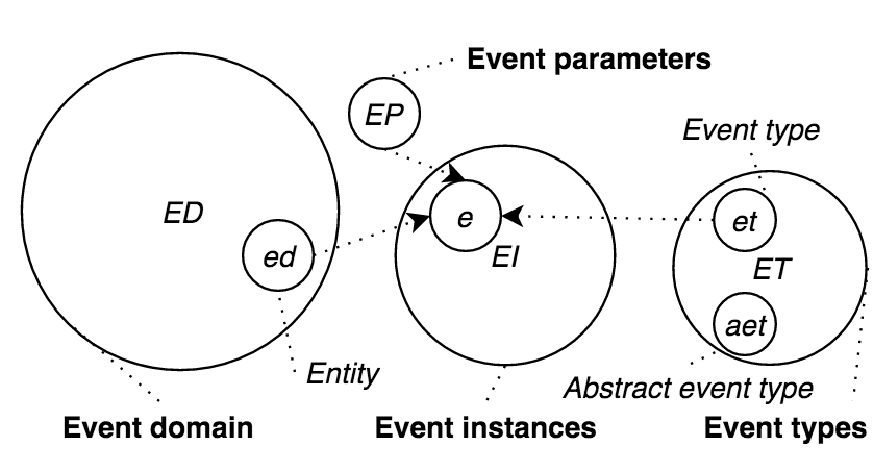
\includegraphics[width=0.7\columnwidth]{eps/event4.eps}
	\caption{Illustration des notions de événements du domaine, des types 
		d'événements, et des instances d'événements.}
	\label{fig:representation_event}
\end{figure} 

Pour décrire le cadre de référence dans lequel les événements se produisent, la 
notion de domaines d'événements est introduite. Un domaine d'événements 
\textit{ED} (\textit{Event Domain}) contient les événements qui respecte les types 
d'événements qui peuvent être spécifiés. Par analogie avec le \gls{DDD}, cet 
espace correspond au contexte borné (cadre d'action) d'un agrégat. À un agrégat 
sont associés des types d'événements \textit{ET} (\textit{Event Type}) particuliers. 
Un \textit{ET} est utilisé pour exprimer un intérêt concret envers les entités d'un 
\textit{ED}. 
Les événements abstraits \textit{aet} (\textit{abstract event type}) sont 
compatibles avec l'\textit{ED}. 
Une instance d'événement \textit{e} -- ou simplement 
événements -- est composée du triplet \textit{ED}, \textit{ET} et \textit{EP}. 
L'ensemble des toutes les instances d'événements possibles est exprimée par 
\textit{EI}. \textit{EP} (Event Parameters) correspond à l'ensemble des paramètres 
que peut avoir l'\textit{EI}. Ainsi, tous les événements sont liés aux intérêts 
d'un~\textit{ED}. La spécification des événements nécessite de 
s'intéresser à tous les types d'événements qui sont utilisés lors de la manipulation 
et la visualisation d'objets 3D dans un \gls{EVC}. La détection d'événement est un 
processus qui permet de récupérer les instances d'événements d'un \textit{ET} en 
particulier. Cela peut être utilisé pour la visualisation de types particulier par 
exemple. Dans 3DEvent, la spécification des événements est calquée sur les 
comportements observés lors des expérimentations des premiers travaux 
\cite{Desprat2015a, Desprat2015b}. 

Le Tableau \ref{tab:extraitevent} ci-dessous, 
présente les événements de l'agrégat Maillage -- extrait du Tableau 
\ref{tab:events} qui résume les 
différents types d'événements de bases construits à partir du framework et les 
agrégats auxquels ils sont associés. Parmi ces événements, l'événement 
\textit{meshAdded} et \textit{meshDropped} semblent être très proches, voire 
identique quant au résultat que l'utilisateur peut obtenir. Cependant, la sémantique 
liée à chacun permet de différencier l'intention de l'utilisateur. 


\begin{table}[ht]
	\centering
	\caption{événements de pour 
		l'agrégat Maillage (extrait de Tab. \ref{tab:events}) }
	\label{tab:extraitevent}
	\begin{tabular}{lll}
		\toprule
		\textbf{événement}& \textbf{Nommage} & \textbf{Description} \\ \midrule
		%\textbf{Agrégat Maillage}  &                      &             \\ \hline
		Maillage ajouté (*)&     meshAdded                 
		&  \begin{tabular}[c]{@{}l@{}} Un maillage a été ajouté dans\\  la Scène à 
			partir d'une géométrie\\ de la 
			bibliothèque \end{tabular}  \\
		Maillage déposé (*) &     meshDropped               
		&      \begin{tabular}[c]{@{}l@{}} Un maillage a été déposé dans 
			\\l'env. 3D de la Scène à 
			partir \\d'une géométrie de la bibliothèque \end{tabular} \\
		Maillage supprimé & meshRemoved       &        \begin{tabular}[c]{@{}l@{}} 
			Un maillage a été 
			supprimé \\de la Scène \end{tabular}      \\
		Maillage translaté &   meshTranslated  	 &    \begin{tabular}[c]{@{}l@{}} Un 
			maillage a 
			subit une translation \\dans la Scène \end{tabular}              \\
		Maillage pivoté &      meshRotated                &    
		\begin{tabular}[c]{@{}l@{}} Un maillage a 
			subit une rotation \\dans la Scène \end{tabular}           \\
		Maillage mis à l'échelle &  meshScaled           &     
		\begin{tabular}[c]{@{}l@{}} Un maillage a 
			subit une homothétie    \\dans la Scène \end{tabular}    \\ 
		\bottomrule
	\end{tabular}
\end{table}

Ce tableau permet de donner un exemple qui reprend la description qui vient d'être 
présentée. L'\textit{ED} correspond donc au \og système de modélisation 3D 
collaborative\fg{}. Dans ce contexte l'agrégat nommé \og Maillage\fg{} réagit à un 
certain nombre de types d'événements comme \textit{meshAdded}, 
\textit{meshDropped} \dots Les événements typés sont produits par l'agrégat en 
prenant en compte les paramètres nécessaires à leur instanciation. Par exemple, 
la production d'un événement \textit{meshTranslated} prend en paramètre le 
vecteur de translation (x,y,z) et la référence de l'identifiant de la scène à laquelle il 
appartient.


Plus généralement, le domaine est la représentation des objets 3D d'un point de 
vue expert. Les objets du domaine représentent les données liées aux 
manipulations 3D sous une forme abstraite (géométrie, position), indépendamment
des besoins du rendu (lumière, matériau \dots). Le framework intègre un 
générateur d'événements pour faciliter l'implantation de nouveau types 
d'événements au plus proche des besoins des utilisateurs dans une application de 
modélisation 3D collaborative (appuyant la sémantique des manipulations).





\subsection{Adaptation des patrons \gls{ES} et \gls{CQRS}}
%TODO mettre l'image representant le cqrs +  celle de la validation des 
%commandes

\begin{figure}[ht]
	\centering
	\includegraphics[width=\columnwidth]{eps/cqrs2.pdf}
	\caption[Modèle de l'architecture client dans 3DEvent]{Modèle de l'architecture 
		client dans 3DEvent : la gestion du cycle de vie des données avec 
		\gls{CQRS} 
		et \gls{ES} dans un navigateur web, des actions utilisateurs à la visualisation 
		en passant par la synchronisation réseau. Issu de \cite{Desprat2017}.}
	\label{fig:cqrs-client}
\end{figure}

La Figure \ref{fig:cqrs-client} montre le déroulement du cycle des opérations du 
modèle au sein de \gls{CQRS}, de l'action utilisateur à la visualisation de son 
résultat. 
Du côté de la partie écriture (partie supérieure -- \textit{write part}), lorsque 
l'utilisateur déclenche une commande à partir de l'interface, la commande et ses 
paramètres sont récupérés et traités par le domaine pour être validés selon les 
règles métiers exprimées par ce dernier. Si la modification est validée, le domaine 
produit ou modifie l'agrégat concerné. Ces modifications sont converties sous 
forme d'événements. Les événements sont ensuite transmis à l'Event Store où ils 
sont stockés 
avant d'être transférés à l'Event Publisher. L'Event Publisher joue le rôle d'interface 
entre la partie écriture et la partie lecture. Il est également responsable de la 
publication des événements sur le bus d'événement Event Bus où sont 
accrochées les différentes projections. Les projections sont nourries a partir des 
événements publiés auxquels elles sont abonnées. Enfin, une Vue (composant
inclus dans l'\gls{IU}) récupère les \glspl{DTO}
contenant les mises à jour à partir d'une projection. La mise à jour d'une Vue peut 
se faire de manière passive -- mode \textit{push} -- (ex. : mises à jour liées à la 
visualisation 3D des modifications des collaborateurs en temps réel) ou active -- 
mode \textit{pull} -- (ex : aller sur une autre scène) selon le contexte.


Le patron \glsreset{ES}\gls{ES} permet de capturer tous les changements d'état 
d'une application sous la forme d'une séquence d'événements. 
Ces événements sont conservés dans un journal d'événements et peuvent être 
rejoués pour retrouver l'état de l'application. 
Les événements représentent des faits immuables qui sont 
seulement ajoutés au journal les un après les autres, ce qui permet des taux de 
transaction élevés et une réplication efficace (cf Section 
\ref{sec:es}). Dans 3DEvent, plusieurs composants d'\gls{ES} sont étendus selon 
les applications :

\begin{itemize}
	\item \textbf{Acteur} Un acteur consomme des événements à partir d'un journal 
	d'événements et produit des événements pour le même journal d'événements. 
	L'état interne dérivé à partir des événements consommés est un modèle 
	d'écriture 
	en mémoire (\textit{in-memory}) et contribue à la partie commande (C) du 
	CQRS\info{reference à la section}.
	\item \textbf{Vue} Une vue est un acteur qui ne fait que consommer des 
	événements à 
	partir du journal d'événements. L'état interne dérivé à partir des événements 
	consommés est un modèle de lecture en mémoire et contribue à la partie 
	requête (Q) du CQRS\info{reference à la section}.
	\item \textbf{Producteur} Un producteur est un acteur qui produit des 
	événements à 
	partir 
	du journal d'événements pour mettre à jour la base de données. L'état interne 
	dérivé 
	à partir des événements consommés est un modèle de lecture en mémoire et 
	contribue à la partie requête (Q) du CQRS\info{reference à la section}.
	\item \textbf{Processeur} Un processeur est un acteur qui consomme des 
	événements 
	à 
	partir d'un journal d'événements et produit les événements traités pour un autre 
	journal d'événements. Les processeurs peuvent être utilisés pour connecter les 
	journaux d'événement au traitement des événements.\info{reference à la 
	section}.
\end{itemize}

%\subsubsection{Collaboration événementielle}

\paragraph{Le journal d'événements}

Les événements produits par un des composants présenté ci-dessus
peuvent être consommés par d'autres de ces abstractions s'ils partagent un 
journal d'événements local ou distribué. Un journal d'événements peut 
fonctionner sur un seul site ou être répliqué 
sur plusieurs sites. 
Le site est considéré comme une zone disponible qui accepte 
l'écriture d'un journal d'événements local même s'il est partitionné sur plusieurs 
sites. Les journaux d'événements locaux situés sur plusieurs sites peuvent être 
connectés par le biais d'un journal d'événements dit \og répliqué\fg{} (copié sur une 
autre réplique) qui a pour responsabilité de préserver l'ordre causal des 
événements.
%\todo{dessin des journaux}  
Les sites peuvent être situés à des endroits géographiquement distincts ou sur 
des nœuds à l'intérieur d'une même grappe (\textit{cluster}) ou encore être sur le 
même nœud mais traités séparément selon les zones 
disponibles qui sont nécessaires au fonctionnement de l'application. 
Les Acteurs et les Processeurs écrivent cependant toujours sur leur journal 
d'événements local. 
Les composants peuvent soit collaborer sur un journal d'événements local sur le 
même site, ou bien au travers d'un journal répliqué sur différents sites.
Il est important de différencier le journal d'événements de la base de données 
(côté serveur) ; la base de données peut ne contenir qu'une partie du journal. 
Une base de données peut également être considérée comme un élément 
complémentaire au journal d'événements, cependant et bien que parfois 
confondus, ils restent bien distincts conceptuellement.
Le journal d'événements commun est la base des échanges pour communiquer 
par le biais d'événements de collaboration. Ce type d'architecture se retrouve dans 
différents cas d'utilisation :
\improve{est ce que cette section est nécessaire?}
\begin{itemize}
	\item \textit{Processus métier distribués.} Les acteurs de différents types 
	utilisent des événements pour communiquer et parvenir à résoudre un problème 
	commun. Bien qu'ils jouent des rôles différents dans le processus métier, ils 
	réagissent à la réception d'événements (programmation réactive) en 
	mettant à jour l'état de l'application et en produisant de nouveaux événements. 
	Cette forme de collaboration est appelée collaboration dirigée par les 
	événements.\improve{ref}
	\item\textit{Réplication d'état d'Acteur.} Les acteurs de même type consomment 
	les événements de chacun pour répliquer l'état interne avec une cohérence 
	causale. Dans 3DEvent, les opérations concurrentes sont autorisées dans 
	l'environnement pour mettre à jour l'état des acteurs répliqués et permettre la 
	résolution interactive de conflit en cas de mises à jour concurrentes et 
	conflictuelles. \improve{miuex 
	expliquer}
	\item \textit{Agrégation d'événement.} Les vues et les producteurs agrègent des 
	événements à partir d'autres composants pour générer des vues spécifiques à 
	l'application.
	La collaboration événementielle apporte de la fiabilité dans la gestion des 
	données dans un système distribué. Par exemple, si un processus distribué 
	échoue à cause d'un problème sur une partie du réseau, le système reprend 
	automatiquement dès les répliques sont à jour.
\end{itemize}

%\paragraph{Bus d'événement}
Les composants souscrivent à leur journal d'événements en s'accrochant au 
\textbf{bus d'événements}.
Les événements nouveaux sont poussés vers les souscripteurs, 
ce qui leur permet de mettre à jour l'état de l'application avec une latence 
minimale. 
Un événement écrit à un endroit est publié de manière fiable aux souscripteurs sur 
ce site et aux souscripteurs des sites distants. 
Par conséquent, les composants qui échangent par le biais d'un 
journal d'événements répliqué communiquent via un bus qui préserve l'ordre causal 
des événements de manière durable et tolérant au partitionnement. De ce fait, les 
services sur les partitions du réseau inter-sites (lien entre les sites) peuvent 
continuer d'écrire des événements localement. La livraison des événements sur 
les sites distants reprend automatiquement lorsque les partitions sont à jour.


Le journal d'événements est répliqué localement et fournit un ordre total des 
événements stockés et appartient à un site. 
Le site est une zone de disponibilité qui héberge un ou plusieurs 
journal d'événements. Les événements d'un journal d'événements sont 
répliqués sur les sites distancts de manière asynchrone. 
Afin de lier des journaux d'événements (localisés sur différents sites) à un journal 
d'événements répliqué, les 
journaux d'événements locaux doivent être accessibles à partir des points 
d'entrées de réplication. De plus, ces points d'entrée doivent être 
connectés entre eux afin de créer un réseau de réplications. 
Un journal d'événements répliqué est représenté par un journal d'événements local 
sur chacun des sites participants.

\info{point d'entrée = network bridge}

Les points d'entrée permettent de gérer un ou plusieurs journaux d'événements. 
Ces journaux sont identifiés pour permettre à la réplication de ne s'intéresser 
qu'aux journaux de même identifiant. 
Les journaux avec différents identifiants sont ainsi isolés les uns des autres et 
leur distribution peut donc varier selon les sites.

Les journaux répliqués fournissent l'ordre causal des événements stockés : l'ordre 
de stockage est le même sur tous les sites, ce qui veut dire que les 
consommateurs qui lisent les événements du journal local vont toujours voir les 
effets avant leurs causes.



\subsection{Cohérence Éventuelle en CQRS}


La \gls{CE}, ou \textit{eventual consistency} en anglais, propose dans un système 
distribué contenant plusieurs répliques d'avoir une coordination lâche entre ces 
répliques. Cela apporte de nombreux avantages en termes de disponibilité, 
tolérance aux fautes et sécurité des données et évite l'intégration de protocoles comme \textit{2 
phase commit} ou de protocoles \textit{Paxos} (consensus) complexifiant les échanges. 
La \gls{CE} introduit l'idée que toutes les répliques se réconcilient au bout d'un 
moment (\textit{forward progression}) pour avoir le même état final. Si le caractère 
vicié d'une information est détecté, le système doit le \og réparer\fg{} pour obtenir 
le bon état. 
\begin{figure} [ht]
	\centering
	\inputTikZ{0.7}{eps/tikz/cap.tex}
	\caption{Théorème CAP et les algorithmes de compromis}
	\label{fig:cap}
\end{figure}
L'ordonnancement des événements durant les mises à jour reste identique lorsque
les événements sont rejoués par la suite car l'ordre issu de l'\gls{ES} est 
déterminée par l'ordonnancement des événements stockés 
localement. Au sein d'une réplique, tous les composants \gls{CQRS} respectent 
cet ordonnancement. L’ordre de stockage des événements répliqués sur des sites 
distincts est cohérent sont ordonnés de manière causale \cite{Lamport1978} : les 
événements liés causalement ont le même ordre sur tous les sites alors que les 
événements concurrents peuvent avoir un ordre différent. Cette propriété est 
importante pour obtenir une cohérence causale forte dans une application qui 
respecte le théorème \gls{CAP} (Figure \ref{fig:cap}).  \blockquote[]{	\textit{The 
largest single 
benefit about 
CQRS is when 
		you start running into 
		problems 
		with the CAP theorem}}{
	\cite{Young2010}
}.
Young justifie ensuite que le lien entre \gls{CAP} et \gls{CQRS} est plus ténu qu'il 
n'y paraît. Même si \gls{CQRS} ne permet pas d'éviter le dilemme de \gls{CAP}, le 
fait que \gls{CQRS} découpe le système en petites parties permet d'ajuster la 
cohérence séparément.

Dans \gls{CQRS}, l'interaction avec plusieurs agents (utilisateurs, services) est 
découplée et subit un traitement réparti 
dont résulte la cohérence éventuelle de l'application. 
Dans la conception d'interaction pour l'interface, la synchronicité peut varier en 
fonction certains contextes. 
Les interactions asynchrones rajoutent souvent des étapes qui polluent l'interface.  
Par exemple, dans le cas de l'interaction suivante : \texttt{soumission de formulaire -> envoi 
asynchrone -> 
message de confirmation}, si l'utilisateur attends que la soumission soit une 
requête qui peut probablement échouer, alors l'asynchronisme se justifie pour être 
capable de fournir une explication à l'utilisateur en cas d'erreur. La probabilité 
d'échec peut être réduite en pré-validant la commande. Si personne d'autre que 
l'utilisateur ne travaille sur l'agrégat, la probabilité d'échec est quasi-nulle. De ce fait, 
l'asynchronicité rajoute une interaction inutile au flux dans le cas où peu de gens 
travaillent sur la même instance d'agrégat.
Par exemple, il est intéressant de rendre l'exécution d'une 
commande synchrone et la mise à jour de la vue asynchrone. Les modèles de 
cohérence sont des décisions liées au métier car ils ont un impact direct sur 
l'expérience utilisateur. 


%Linéaire (strong consistency)
%one version replace another -- one parent and one children in the sequence
%each version is immutable 
%each version has an identity
%each new version is a replacement of the previous (earlier)
%directed acyclic graph (eventual consistency)
%each version may have one or more parent
%each parent may have one or more parent
%each parent may have children with different parents
%each version is immutable
%each version has an identity
%
%each version may be viewed as one of many replacement version for its parents
%
%version are immutable and (should) have immutable names


%\begin{algorithm}[caption="titi"]
%	
%    saveEvents(itemId:string, events:EventMessage[], expectedVersion:number) 
%{\\
%    	var eventDescriptors:EventDescriptor[] = 
%this.eventDescriptorsByAggregate[itemId];\\
%    	if (!eventDescriptors) {\\
%    		eventDescriptors = this.eventDescriptorsByAggregate[itemId] = [];\\
%    	} else if (eventDescriptors.length > 0 \&\& 
%eventDescriptors[eventDescriptors.length\\ - 1].version != expectedVersion \&\& 
%expectedVersion != -1) {\\
%    	throw new Error("ConcurrencyException");\\
%    }
%    var i = expectedVersion;\\
%    events.forEach((event:EventMessage) => {\\
%    	i++;\\
%    	event.version = i;\\
%    	var eventDescriptor = {id: event.AggregateId(), version: i, eventData: 
%event};\\
%    	eventDescriptors.push(eventDescriptor);\\
%    	this.\_publisher.publish(event);\\
%    	this.\_network.publishEvent(event);\\
%    });
%}
%\end{algorithm}
\subsection{Potentielles applications et autres utilisations}
La conception et l'implémentation d'une plateforme comme 3DEvent qui est 
asynchrone, distribuée et orientée événements  (notamment la persistance) peut 
être appliquée à différents champs.
\begin{description}
	\item[GIT-like app] Les solutions pour faire de la gestion de version, comme 
	MeshGit~\cite{Denning2013} par exemple qui fait du
	\textit{diff and merge} de maillages polygonaux pour des données 3D, 
	sont rarement implémentées (a fortiori en 
	temps-réel) sur des plateformes web à cause du coût et de la complexité que 
	cela peut apporter dans des architectures traditionnelles. 3DEvent peut 
	reconstruire n'importe quel état antérieur grâce à son architecture orientée 
	événements et indiquer les différences entre deux états.%\todo{acyclic graph}
	
	\item[Scenarii et \textit{path recording}] Pour des jeux sérieux, les graphistes 
	3D ou des études d'ergonomie, cette fonctionnalité est particulièrement 
	pertinente. Le \gls{framework} peut proposer une comparaison entre deux traces 
	laissées par un ou plusieurs utilisateurs. Dans le cas où les utilisateurs ont la 
	même tâche à réaliser, il est facile de faire la différence entre deux réalisations 
	pour comparer, analyser et montrer les résultats	pour des raisons 
	pédagogiques ou pour relever des habitudes (de travail) par exemple. Dans 
	l'exemple du jeu sérieux, il est possible de comparer la trace utilisateur à la trace experte 
	et permettre de rejouer le même scénario plusieurs fois facilement pour 
	observer l'évolution. Ce type de fonctionnalité est intrinsèque à 3DEvent. 
	
	\item[Traçage utilisateur et \textit{crowdsouring}] 3DEvent peut se révéler être 
	un bon outil pour enregistrer la trace d'un utilisateur lorsqu'il navigue dans la 
	scène. L'enregistrement du chemin de la caméra et des actions de l'utilisateur 
	sous la forme d'événements sont des informations 
	"issues de la foule" (\textit{crowdsouring}). En utilisant un processus 
	d'apprentissage, il est possible de proposer de meilleurs chemins, repérer des 
	points d'intérêt, ou même proposer des résumés de scène générés à partir des 
	traces des collaborateurs (que s'est-il passé depuis la dernière connexion du 
	collaborateur X ?).
	\item[Audit et outils de surveillance de données 3D] L'\gls{ES} fournit un 
	mécanisme 
	d'audit intégré qui assure la cohérence des données transactionnelles. Utiliser 
	ce mécanisme pour faire un audit ou surveiller en temps réel l'activité de 
	l'application peut fournir une meilleure compréhension du travail d'équipe ainsi 
	que l'évolution de la conception. Cela peut permettre de repérer (avec du 
	\gls{CEP}) et corriger certaines fonctionnalités afin d'améliorer l'ergonomie de 
	l'application. Par exemple, si un événement est anormalement représenté dans 
	le journal des événements, il sera possible de lever une alerte facilement.
\end{description}
%\begin{figure}[htb]
%	\centering
%	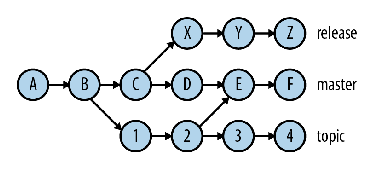
\includegraphics[width=0.3\columnwidth]{gitgraph}
%	\caption{Exemple d'arbre de commits Git}
%	\label{fig:git}
%\end{figure}
\subsection{Bilan}

Le modèle orienté événement pour la modélisation 3D collaborative présenté dans 
cette section intègre les besoins métiers par différents aspects. Le suivi des 
directives liées au \gls{DDD} permet de mieux cerner les règles 
métiers pour les intégrer dans \gls{CQRS}. 

La description de la typologie des 
événements manipulés insiste sur le compartimentage des objets métiers. La 
modélisation 3D collaborative est minutieusement étudiée pour en dégager les quatre 
agrégats fondamentaux (la scène, le maillage, la géométrie et l'utilisateur) et les 
types d'événements qui leurs sont associés. Cette étape introduit des différences 
fines sur les événements qui sont produits à partir d'un agrégat. 
Cet aspect est notamment intéressant pour l'observation et la surveillance du 
contenu des sessions collaboratives développés en Section 
\ref{sec:flexviz}. \todo{attention garder le bon endroit}
Les composants du patron \gls{CQRS} favorisent le découplage de l'application 
pour obtenir une gestion de la cohérence plus fine. 

La partie \gls{ES} s'intéresse à la sauvegarde des événements dans un journal 
d'événement, et notamment dans le cas des applications distribuées en proposant 
un mécanisme de synchronisation pour détecter les conflits. La fonction principale 
de cette partie est de permettre de recréer un état de l'application cohérent en 
intégrant implicitement une gestion de version des événements.

Ce modèle introduit le cadre de travail pour utilisateur expert en manipulation 3D, il 
peut être facilement adapté pour différents types d'applications et étendu à 
d'autres utilisations. 
Pour mettre en avant l'expertise de chacun et profiter de 
toutes les ressources apportées par un utilisateur, une communication efficace de 
ces événements pour la collaboration doit désormais être établie entre les 
collaborateurs.